\section{Channels}
Una delle piu importanti feature del linguaggio go sono i canali.\newline 
Un canale si puo visualizzare come un tunnel che viene utilizzato per comunicare tra due punti, il dato quindi viene inviato da un estremita all'altra, questo e' utile per comunicare tra goroutine diverse.

\begin{figure}[h!]
    \centering
    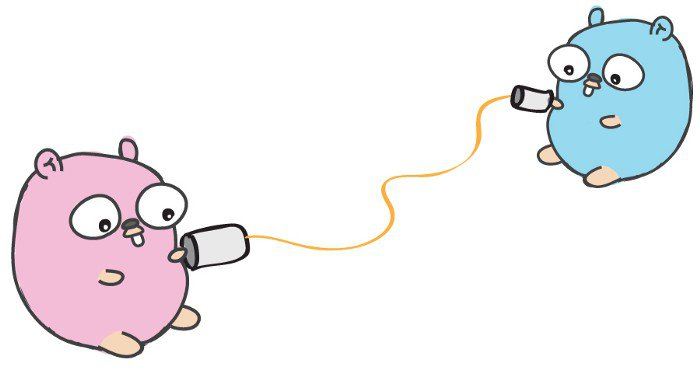
\includegraphics[width=5cm]{channel.jpg}
    \caption{channel}
    \label{fig:title}
\end{figure}

Come funzionano? Iniziamo dalla creazione, i canali si creano utilizzando il metodo make e il tipo chan seguito dal tipo di messaggio che verra scambiato all'interno di esso, quello che otteniamo e' un puntatore ad un canale che risiede nell'heap del nostro programma: \newline

\begin{lstlisting}
ch := make(chan int, 3) //buffered channel
ch := make(chan int)    //unbuffered channel
\end{lstlisting}

\subsection{Struttura di un canale (hchan)} 

\begin{figure}[h!]
    \centering
    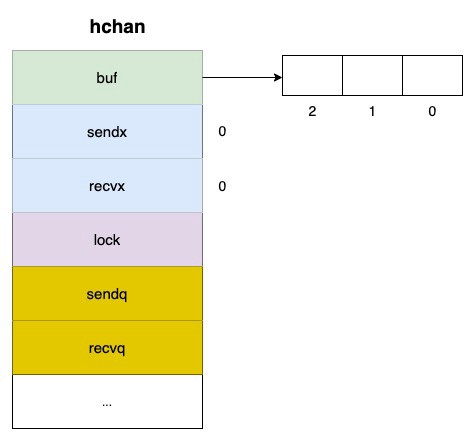
\includegraphics[width=6cm]{sections/channel-struct.jpeg}
    \caption{struttura di un canale}
    \label{fig:title}
\end{figure}

Come vediamo sopra il canale ha: 
\begin{itemize}
    \item buffer: dove andiamo a raccogliere gli oggetti che inseriamo all'interno del canale
    \item sendx: indice che indica che una goroutine sta aspettando per inviare un oggetto
    \item recvx:
    indice che indica che una goroutine sta aspettando per ricevere un oggetto
    \item lock: il mutex per accedere al canale in modo concorrente
    \item sendq: la queue dove vengono messe in waiting le goroutine che non riescono a trovare il canale vuoto
    \item recvq: la queue dove vengono messe in waiting le goroutine che non riescono a trovare un messaggio all'interno del canale
\end{itemize}

\vspace{1cm}

Abbiamo creato due canali entrambi che possono scambiare messaggi di tipo int, i canali vengono creati per loro natura unbuffered, ovvero \textbf{bloccanti}, significa che prima di poter ricevere un altro messaggio da inviare dovra inviare quello gia presente all'interno del canale, mentre al contrario un canale buffered potra contenere piu messaggi ma quando anche lui sara pieno bisognera aspettare che qualcuno prenda il messaggio in uscita prima di poter inserire un nuovo messaggio \newline
Come si utilizzano i channel? I valori vengono inviati e ricevuti tramite l'utilizzo dell'operatore \textbf{$\rightarrow$}:

\begin{lstlisting}

//unbuffered channel
ch := make(ch int) //creiamo il canale
ch <- 42 //inviamo 42 sul canale
n := <- ch //riceviamo dal canale 42

//nel caso di buffered channel
ch := make(ch int, 10)
ch <- 42
ch <- 12
ch <- 3

fmt.Println(<- ch)
fmt.Println(<- ch)
fmt.Println(<- ch)

/*
ci aspettiamo un output di questo tipo:
42
12
3
*/

\end{lstlisting}

\subsection{Worker pool}
Ma perche i channel sono importanti? Immaginiamo per esempio di avere delle task e di doverle passare ad un worker per essere eseguite, quindi dovremo implementare una worker pool 

\begin{figure}[h!]
    \centering
    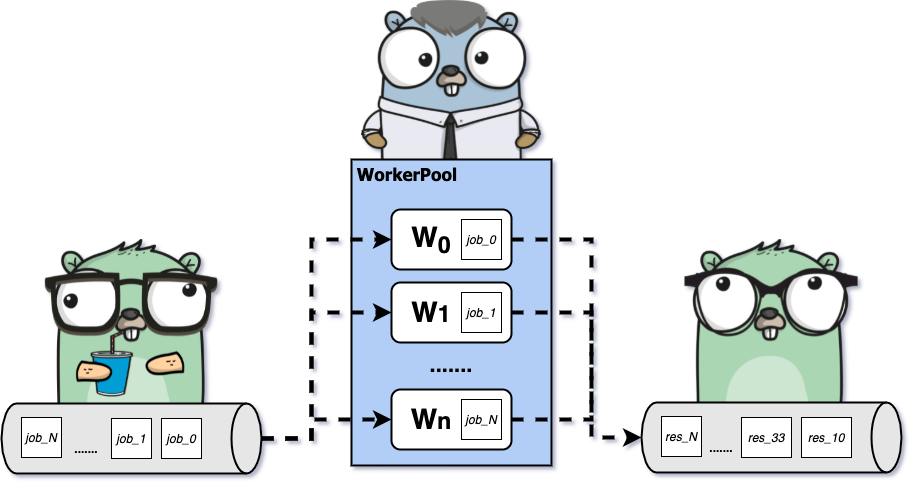
\includegraphics[width=8cm]{sections/worker-pool.png}
    \caption{worker pool}
    \label{fig:my_label}
\end{figure}

Con il go e' molto semplice farlo tramite l'utilizzo dei canali: \newline

\begin{lstlisting}
package main

func worker(ch) {
    for {
        //ricevo il task
        task := <- taskCh
        process(task)   //eseguo il task
    }
}

func main() {
    //creo il canale, in questo caso un buffered channel
    ch := make(chan Task, 3)
    
    //creazione dei worker
    for i := 0; i < numWorkers; i++ {
        go worker(ch)
    }
    
    hellaTasks := getTasks()
    
    //invio della task al worker
    for _, task := range hellaTasks {
        taskCh <- task
    }
}
\end{lstlisting}

Tramite l'utilizzo dei canali il codice rimane piu pulito, leggibile, veloce da scrivere e performante.

